\documentclass[oneside,10pt]{book}

\usepackage{cdtBook}
\usepackage{usecases}

\title{Análisis de requerimientos del proyecto Deportivo San Pancho}
\subtitle{Sistema de Control del Centro Deportivo, Módulos de Cliente, Área, Sucursal, Instructor y Curso}
\author{Equipo: RGBA Group}
%\organization{Escuela Superior de Cómputo, IPN}


%%%%%%%%%%%%%%%%%%%%%%%%%%%%%%%%%%%%%%%%%%%%%%%%%%%%%%%%%%%%%%%%
\begin{document}

\maketitle
\thispagestyle{empty}

\frontmatter
\tableofcontents

\mainmatter
%=========================================================
\chapter{Introducción}
\cfinput{intro}

%=========================================================
\chapter{Modelo de Negocios}

\cfinput{reglas}

%=========================================================
\chapter{Modelo de Casos de Uso}

\begin{figure}[htbp!]
		\centering
			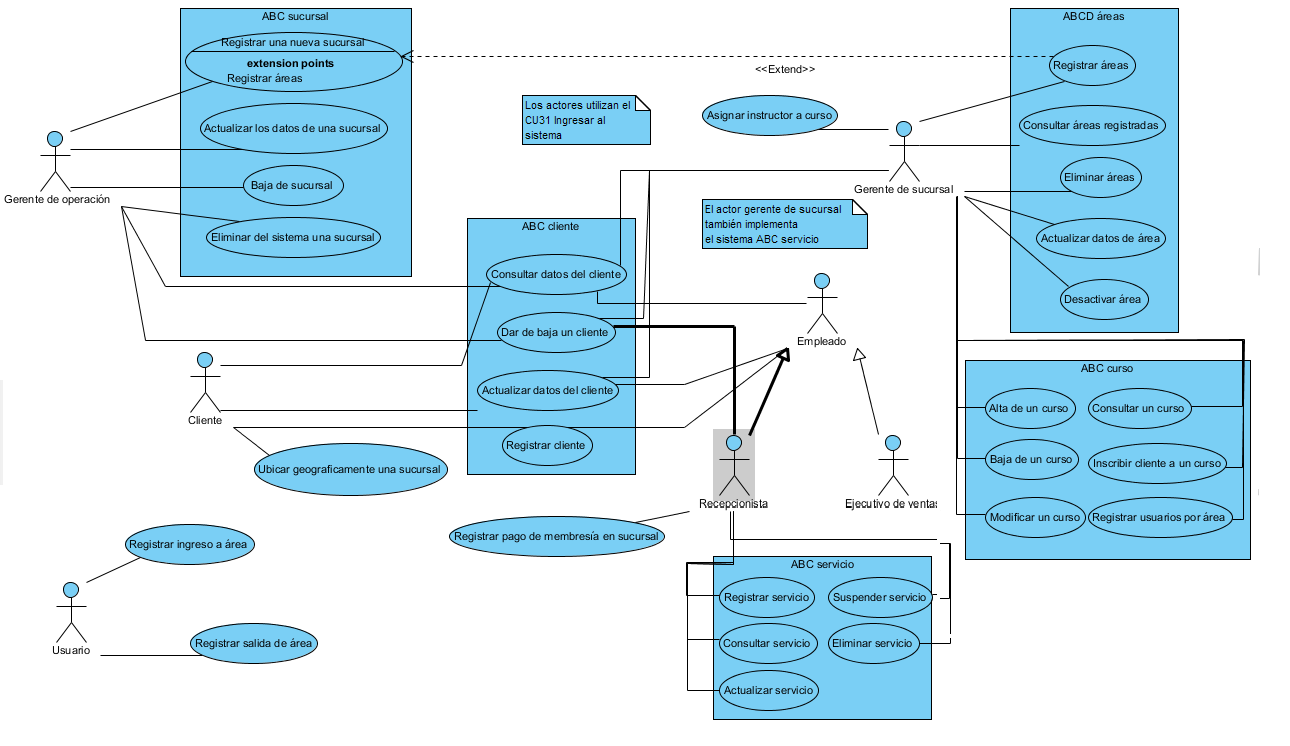
\includegraphics[width=1.2\textwidth]{images/CasosDeUso}
		\caption{Diagrama de Casos de Uso del sistema.}
	\end{figure}
	
\cfinput{cu/cu01}
\cfinput{cu/cu02}
\cfinput{cu/cu03}
\cfinput{cu/cu04}
\cfinput{cu/cu06}
\cfinput{cu/cu07}
\cfinput{cu/cu08}	
\cfinput{cu/cu09}
\cfinput{cu/cu10}
\cfinput{cu/cu11}
\cfinput{cu/cu12}
\cfinput{cu/cu13}
\cfinput{cu/cu14}
\cfinput{cu/cu15}
\cfinput{cu/cu21}
\cfinput{cu/cu22}
\cfinput{cu/cu23}
\cfinput{cu/cu24}
\cfinput{cu/cu25}
\cfinput{cu/cu26}
\cfinput{cu/cu28}
\cfinput{cu/cu29}
\cfinput{cu/cu30}
\cfinput{cu/cu31}
\cfinput{cu/cu32}
\cfinput{cu/cu33}
\cfinput{cu/cu34}
\cfinput{cu/cu35}
\cfinput{cu/cu36}
\cfinput{cu/cu37}

%%=========================================================
\chapter{Modelo de la Interacción}

{\color{UCInterfaceColor} 
	Esta sección se queda deliberadamente en blanco debido a que el diseño de las interfaces dependerá de la plataforma a utilizar por cada equipo.\\	
}
\cfinput{Pantallas/IU21_0}
\cfinput{Pantallas/IU21_1}
\cfinput{Pantallas/IU21_2}
\cfinput{Pantallas/IU22_1}
\cfinput{Pantallas/IU23_1}
\cfinput{Pantallas/IU24_1}
\cfinput{Pantallas/IU25_1}
\cfinput{Pantallas/IU23}
\cfinput{Pantallas/IU24}
\cfinput{Pantallas/IU3}
\cfinput{Pantallas/IU1}


%=========================================================
\chapter{Modelo del Dominio del problema}

	\begin{figure}[htbp!]
		\centering
			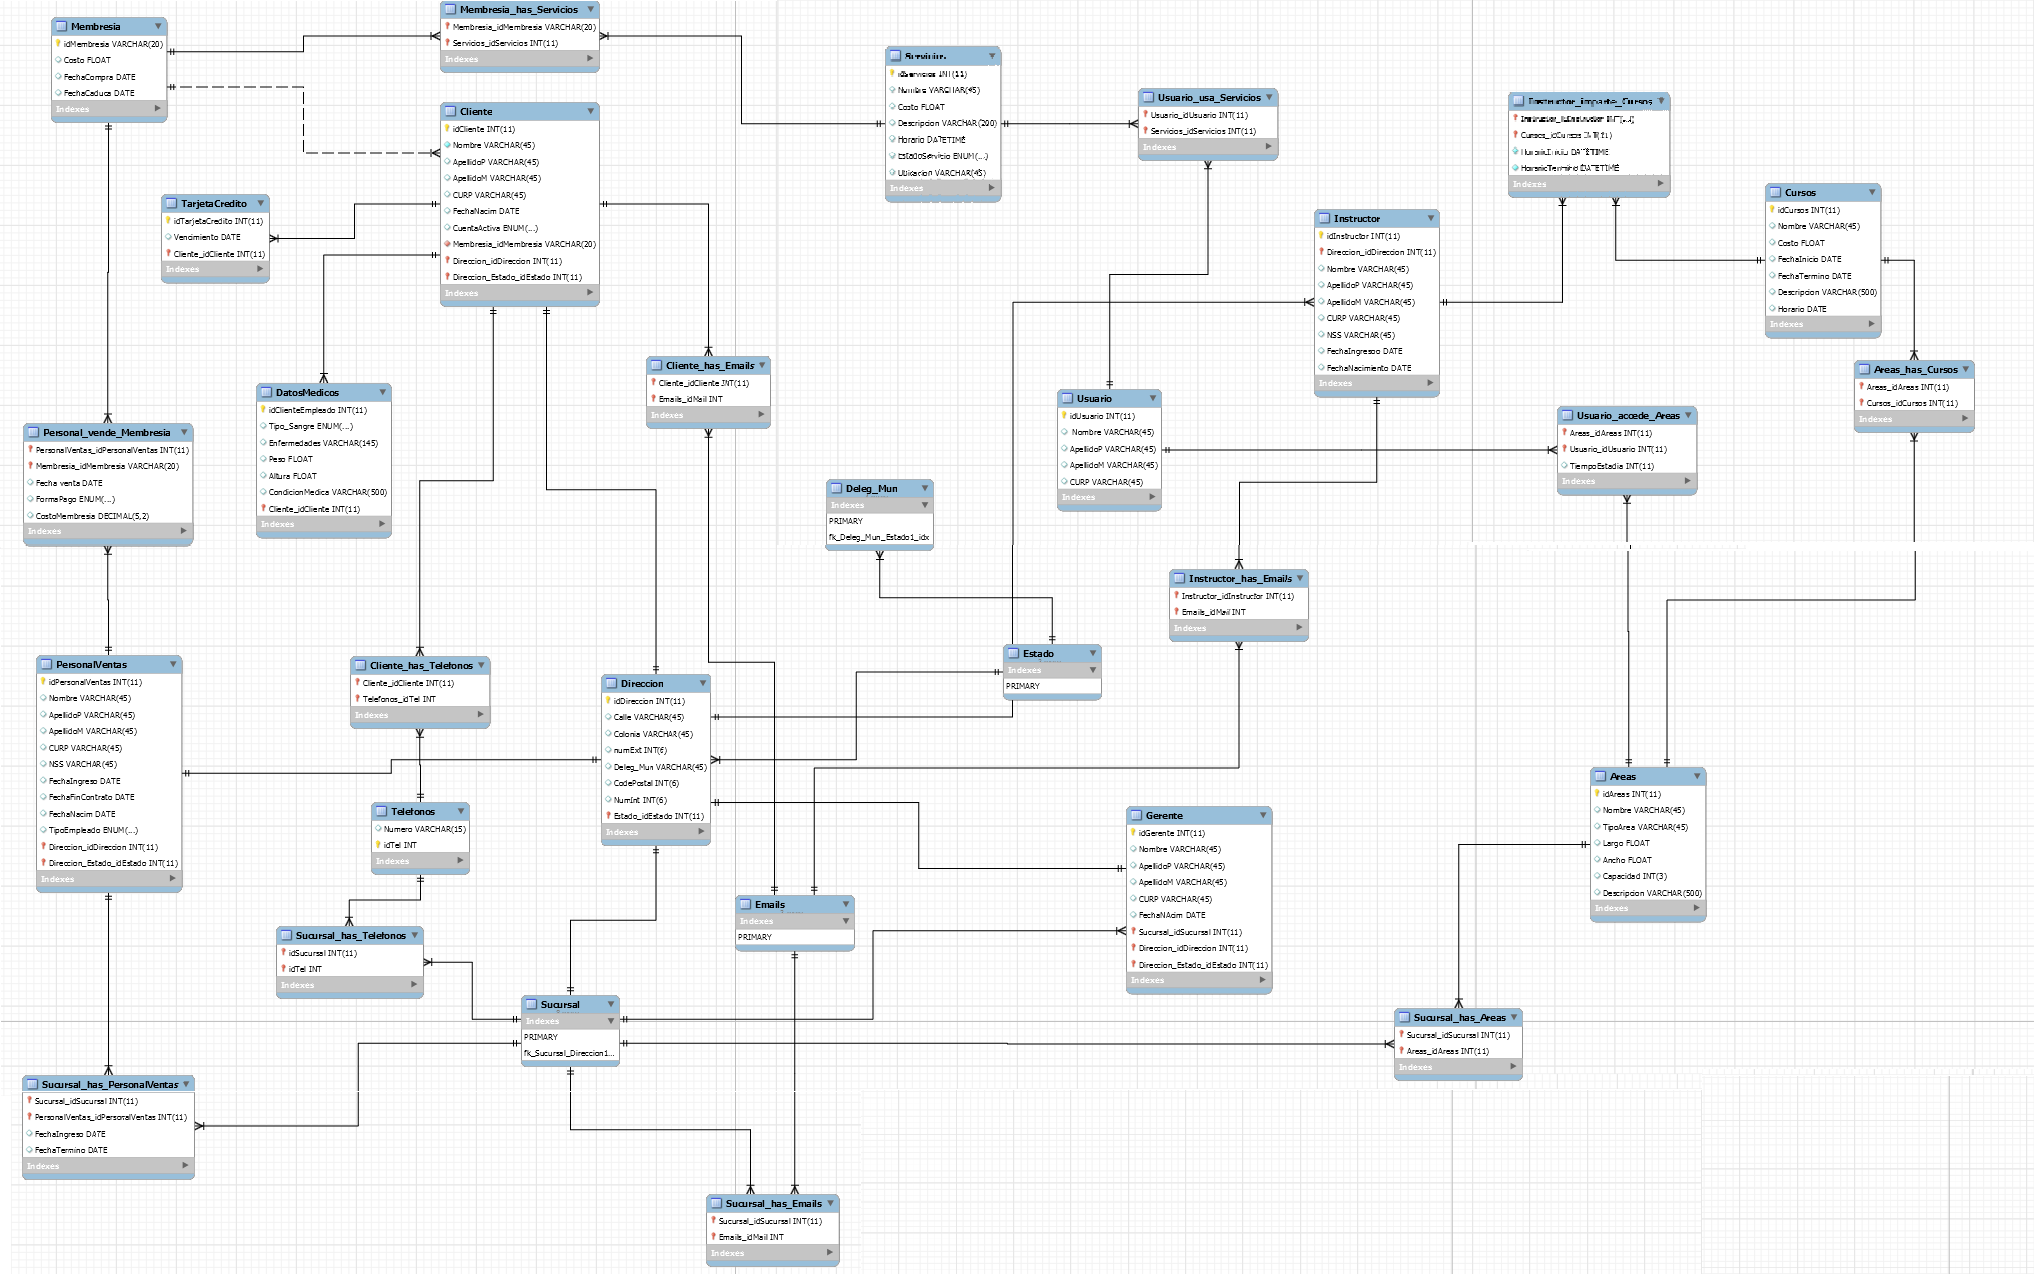
\includegraphics[width=1.2\textwidth]{images/baseDeDatos}
		\caption{Diseño de la Base de Datos.}
	\end{figure}
	
\end{document}
